\chapter[Exemple concret]{Exemple concret de mise en place des tests d'acceptation dans un environnement agile}
\thispagestyle{fancy}
\label{chap:exemples}
Dans cette section nous allons voir comment mettre une stratégie de tests fonctionels d'acceptation dans une entreprise ainsi que les outils utilisés pour la mise en place de cette stratégie.

\section{Etat de l'art des outils BDD ATD}
\label{sec:etat}
Il existe plusieurs outils de tests d'acceptation qui sont disponibles sur le marché. Nous allons voir dans cette section les outils les plus utilisés et leurs avantages et inconvénients.

En termes de langages de programmation plusieurs incluent des bibliothéque et des frameork  de tests ce qui veut dire que les tests ne seront pas développé de zéro.  le choix d'un langage de programmation dépend donc de chaque entreprise et de chaque appllication en effet il est préferable de tester avec le meme langage de programmation avec laquelle l'application est écrite.

\begin{itemize}

\item  Java avec Cucumber-JVM
\item  Java avec JBehave
\item  JavaScript avec Cucumber.js
\item  Python avec Behave
\item  .NET avec SpecFlow

\end{itemize}

Dans la majorité de ces outils les tests sont écrits dans un fichier de format ".feature" "fig" où à chaque étape on peut définir une action, une assertion ou une vérification.

il existe aussi des outils de tests qui ne nécessite pas de langage de programmation. comme par exemple Selenium qui enregistre les actions de l'utilisateur et génère un script de test à partir de ces actions.

le code associé à un fichier de fonctionnalité (fichier.feature) est défini dans des classes d'étapes didiées comme DefFonctionnali1 et DefFonctionnali2 dédiées. Ces classes contiennent les méthodes qui correspondent aux étapes décrites dans le fichier .feature.
exemple:

\begin{lstlisting}[language=Java]
    @Given("je suis sur la page d'acceuil")
    public void jeSuisSurLaPageDAcceuil() {
        \\ ici le code du test
    }
\end{lstlisting}
c'est ainsi que sont associés les fichiers .feature et differentes classes et méthode java.
Nous pourrons également rajouter des parametres ou des jeux de données dans les fichiers .feature \parencite{BddInAction}.
Apres l'éxecution des tests quelques outils integrent la possibilité de générer des rapports de tests qui permettent de visualiser les résultats des tests. Ces rapports sont souvent générés au format HTML pour la visualisation humaine ou au format xml ou json pour des traitement supplémentaire comme par exemple l'envoie vers un outils de gestion des projets.

\begin{center}
    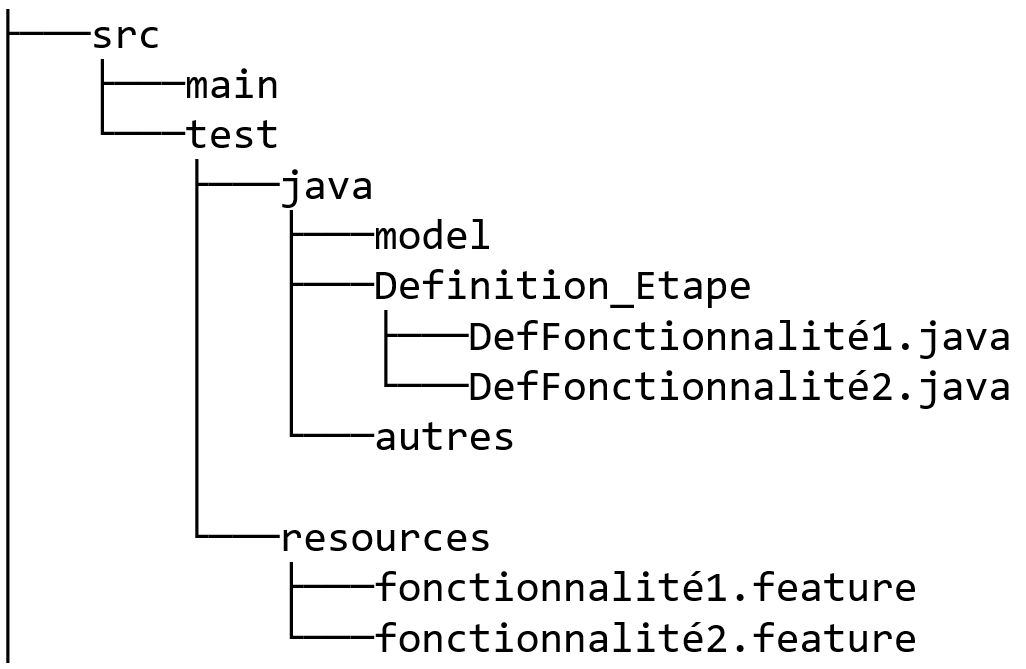
\includegraphics[width=0.5\textwidth]{filetree.png}

\end{center}


\section{Organisation des équipes et bonnes pratiques de tests }
\label{sec:organisation}

\begin{center}
    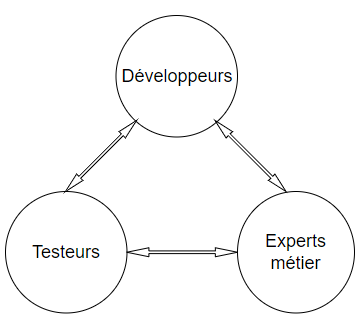
\includegraphics[width=0.5\textwidth]{interaction.png}
    \linebreak
fig:comment les choses doibe
\end{center}

Ici je vais élaborer les points suivants \parencite{cftl} :


Éviter de faire une surqualification.
Sélectionner soigneusement les tests de régression.
Maintenir la campagne de tests de régression.
Mettre à jour les cas de tests dès qu'ils sont affectés par un nouveau développement ajouté au produit.
Supprimer les tests qui se révèlent inutiles.
Élargir les campagnes avec des tests couvrant de nouvelles fonctionnalités.
Supprimer les tests les moins importants.


Lutter contre le paradoxe des pesticides en utilisant des tests exploratoires.
Mettre en place des outils communs pour les tests.
Comprendre l'application et savoir quoi automatiser.
Choisir les bons outils d'automatisation.
Tous les tests doivent être indépendants.
Configurer des rapports détaillés d'automatisation des tests.
Éviter les scénarios d'automatisation trop techniques et écrits par les développeurs.
Les scénarios automatisés peuvent servir de documentation vivante pour l'application.

Outils de gestion des tests:
Utiliser des outils de gestion des tests (Zephyr for Jira, TestRail, Xray).
Ils intègrent un support de base pour BDD.
Ils ne proposent pas d'intégration avec Git ou de documentation vivante.


\section{Outils de gestion de projet}
\label{sec:outils}
Dans un projet de test, les équipes de développement, de test et les experts métiers collaborent sur un outil de gestion de projet pour déterminer une stratégie de test. Chacun apporte son expertise en matière de développement dirigé par les tests (ATDD). Ils planifient les scénarios de test, les fonctionnalités à tester et les parties à automatiser. Une fois les fonctionnalités développées, les tests sont exportés vers le dépôt de code, où ils sont exécutés, et les résultats sont examinés et revus sur l'outil de gestion de projet.

En plus de tester les nouvelles fonctionnalités, il est important de s'assurer que les modifications apportées n'ont pas affecté les fonctionnalités existantes. C'est ce que l'on appelle les tests de non-régression. Ces tests sont idéalement déjà développés, mais peuvent nécessiter une rectification. Dans ce cas, on utilise un outil d'intégration continue pour garantir la qualité du logiciel.
.................
................. Ici je vais expliquer comment on pourra lier le projet de test avec l'outil de gestion (exemple de Jira)

\section{cycle de test et integration continue}

Ici je vais parler des outils d'integration continue comme par exemple jenkins ou gitlab CI pour automatiser le lancement des tests apres les commits des develppeurs ou apres la création d'un nouveau ticket dans l'outil de gestion de projet.
